\documentclass{article}
\usepackage{amsmath}
\usepackage{amssymb}
\usepackage{graphicx}
\usepackage{hyperref}
\usepackage[version=4]{mhchem}


\begin{document}
In \(\triangle A B C, D, E\) are points on \(A C B\), and \(A B\), respectively. \(C E\) and \(C D\) meet at \(M . \angle D B C=\angle A . B M=M D\). Prove that \(\frac{B C^{2}}{A C^{2}}=\frac{B E}{A E}\).

Solution:
Method 1:\\
\centering
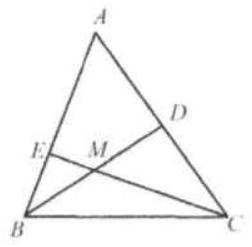
\includegraphics[width=\textwidth]{images/115.jpg}

Since \(\angle D B C=\angle A, \angle A C B=\angle B C D, \triangle A B C \sim \triangle B D C\).

\[
\frac{B C}{C D}=\frac{A C}{B C} \quad \Rightarrow \quad \frac{B C^{2}}{A C^{2}}=\frac{C D}{A C}
\]

Draw \(D F / / B E\) to meet \(C E\) at \(F . \triangle A C E \sim \triangle D C F\).\\
\(\frac{C D}{A C}=\frac{D F}{A E}\)\\
We know that \(\triangle B E M \sim \triangle D F\).\\
\centering
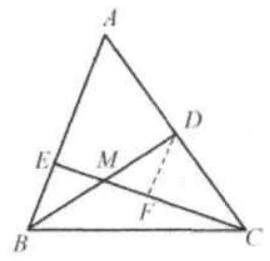
\includegraphics[width=\textwidth]{images/115(1).jpg}

So we have \(\frac{D F}{M D}=\frac{B E}{B M}\) or \(\frac{D F}{M D}=\frac{B E}{M D}\).\\
So \(D F=B E\).\\
Thus \(\frac{B C^{2}}{A C^{2}}=\frac{C D}{A C}=\frac{D F}{A E}=\frac{B E}{A E}\).\\
Method 2:\\
Since \(\angle D B C=\angle A, \angle A C B=\angle B C D, \triangle A B C \sim \triangle B D C\).

\[
\frac{B C}{C D}=\frac{A C}{B C} \quad \Rightarrow \quad \frac{B C^{2}}{A C^{2}}=\frac{C D}{A C}
\]

Draw \(B N / / A C\) to meet the extension of \(C E\) at \(N\). Since\\
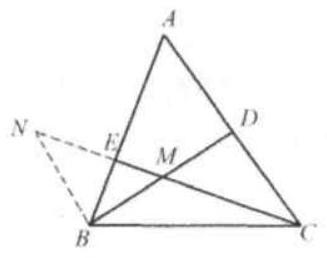
\includegraphics[width=\textwidth]{images/115(2).jpg} \(\angle N M B=\angle C M D, B M=M D, \angle N B M=\angle C D M, \triangle N M B \cong \triangle C M D\). Then \(B N=\) \(C D\).\\
Since \(\angle N=\angle E C A, \angle N E B=\angle C E A, \triangle N E B \sim \triangle C E A\).\\
So \(\frac{B N}{A C}=\frac{B E}{A E} \quad \Rightarrow \quad \frac{C D}{A C}=\frac{B E}{A E}\).


Therefore, \(\frac{B C^{2}}{A C^{2}}=\frac{B E}{A E}\).

Method 3:\\
Since \(\angle D B C=\angle A, \angle A C B=\angle B C D, \triangle A B C \sim \triangle B D C\).

\[
\frac{B C}{C D}=\frac{A C}{B C} \quad \Rightarrow \quad \frac{B C^{2}}{A C^{2}}=\frac{C D}{A C}
\]

Draw \(A P / / B D\) to meet the extension of \(C E\) at \(P\).\\
We know that \(\triangle A E P \sim \triangle B E M(A A) \cdot \frac{B M}{A P}=\frac{B E}{A E}\).\\
\centering
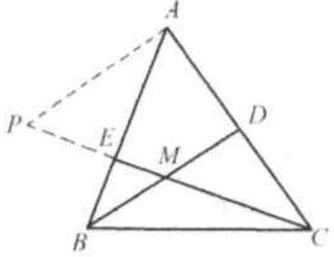
\includegraphics[width=\textwidth]{images/116.jpg}

We know that \(\triangle A C P \sim \triangle D C M(A A) \cdot \frac{C D}{A C}=\frac{D M}{A P}\).\\
Since \(B M=M D, \frac{C D}{A C}=\frac{B M}{A P}=\frac{B E}{A E}\).\\
Therefore, \(\frac{B C^{2}}{A C^{2}}=\frac{B E}{A E}\).


\end{document}
